\documentclass[11pt, a4paper]{article}

\usepackage{amsmath, amsthm, amssymb}
\usepackage[top=0.8in, bottom=0.8in, left=0.8in, right=0.8in]{geometry}
\usepackage{graphicx}
\usepackage{float}
\usepackage{booktabs}
\usepackage{caption}
\usepackage{xcolor}
\usepackage[unicode, colorlinks=true, linkcolor=blue!70!black, urlcolor=blue!70!black, filecolor=red!75!black]{hyperref}
\usepackage{tikz}
\usetikzlibrary{arrows.meta, positioning, shapes.geometric, calc, patterns}
\usepackage[bidi=bidi]{babel}
\babelprovide[import, main]{hebrew}
\babelprovide[import]{english}
\usepackage{fontspec}
\babelfont{rm}{Times New Roman}
\babelfont{sf}{Arial}
\babelfont{tt}{Courier New}

\captionsetup{font=small, labelfont=bf, skip=4pt}

\newtheorem{theorem}{משפט}
\newtheorem{proposition}{טענה}
\newtheorem{assumption}{הנחה}
\newtheorem{remark}{הערה}

\title{\vspace{-1.2em}\Large\textbf{ניווט \foreignlanguage{english}{I-Bug} חסין תחת מתקפת התחזות אותות לסירוגין}\\
\large\textbf{גרסה מונגשת ומאוירת להבנת המתמטיקה והמונחים במאמר המדעי}\\[0.4ex]
\normalsize\foreignlanguage{english}{\textbf{Resilient I-Bug Navigation under Intermittent Signal Spoofing (Illustrated Accessible Edition)}}}

\author{
  \textbf{צוריאל ויזל} \quad \textbf{אברהם גז} \\
  \small מנחה: ד"ר אנדריי ז'יטניקוב $\cdot$ הטכניון -- מכון טכנולוגי לישראל
}
\date{}

\begin{document}

\maketitle

\begin{abstract}
\noindent
\textbf{על מה המאמר במשפט אחד?} דמיינו רובוט פשוט מאוד שצריך להגיע למגדל שידור בתוך מבוך חשוך (ללא \foreignlanguage{english}{GPS} וללא מפה), כשהחיישנים היחידים שלו הם "חיישן מישוש" לקירות וחיישן שמודד את עוצמת האות מהמגדל (כמו במשחק "חם-קר"). במאמר זה אנו מראים איך "מגדל תוקף" שמדליק ומכבה אות מזויף יכול לשגע את הרובוט וללכוד אותו בלולאה אינסופית — וחשוב מכך, איך הרובוט יכול להשתמש בחוקי הפיזיקה של המהירות של עצמו כדי לחשוף את התרמית ולנצח, בלי להוסיף אף חיישן חדש!

\smallskip
\noindent
\textbf{התקציר המדעי המונגש:}
רובוטים אוטונומיים מינימליסטיים (פשוטים ודלי-חיישנים) הפועלים בסביבות חסומות \foreignlanguage{english}{GPS} מסתמכים על מידע מקומי מהחיישנים שלהם במקום על מיקום גלובלי או \textbf{אודומטריה} (ספירת סיבובי גלגלים לחישוב מרחק). אלגוריתם ה-\foreignlanguage{english}{I-Bug} מבטיח מתמטית שהרובוט יגיע למטרה באמצעות חיישן מגע וחיישן \textbf{סקלרי} (חיישן שמחזיר מספר בודד — עוצמה — ללא כיוון) בלבד. אולם, כאשר ישנם מספר משדרים במרחב והמקלט מודד את \textbf{הסכום החיבורי} של העוצמות שלהם, הרובוט חשוף למתקפות \textbf{התחזות (\foreignlanguage{english}{Spoofing})} לסירוגין. משדר תוקף שפועל לסירוגין מעוות את כיוון העלייה בעוצמה (\textbf{הגרדיאנט}) במרחב הפתוח ויוצר שיאי עוצמה מזויפים לאורך קירות של מכשולים, מה שלוכד רובוט \foreignlanguage{english}{I-Bug} רגיל בהקפות אינסופיות סביב מכשולים. אנו מציגים \textbf{מסנן אנומליות} (גלאי חריגות) המבוסס על מהירות התנועה של הרובוט ושתי אסטרטגיות התגוננות — אסטרטגיה \textit{זהירה} (\foreignlanguage{english}{Cautious}) המשמרת במדויק את מסלול התנועה הבטוח של הרובוט התקין, ואסטרטגיה \textit{אינרציאלית} (\foreignlanguage{english}{Inertial}) מהירה שממשיכה לנוע "על עיוור" בזמן ההפרעה. אנו מוכיחים מתמטית שהאסטרטגיה הזהירה תמיד תשחזר את ההצלחה של רובוט ללא תקיפה, ומסבירים תופעה מפתיעה של \textbf{תהודה (\foreignlanguage{english}{Resonance})} שבה סנכרון זמנים בין הקפת מכשול לבין קצב ההבהוב של התוקף עלול ללכוד את האסטרטגיה האינרציאלית. בניסויי סימולציה על פני $1,000,000$ מבוכים אקראיים, הרובוט התמים (\foreignlanguage{english}{Naive}) מצליח רק ב-$54.68\%$ מהמקרים, האסטרטגיה האינרציאלית מצליחה ב-$99.61\%$ תוך קיצור זמן ההגעה ב-$20.5\%$, והאסטרטגיה הזהירה משיגה $\mathbf{100.00\%}$ הצלחה.
\end{abstract}

\section*{מדריך קריאה: מילון סימונים מתמטיים ומונחים (לפני שמתחילים)}
כדי שתוכלו לקרוא הן את הגרסה הזו והן את המאמר המדעי המקורי בקלות, הנה פירוש הסימונים המתמטיים המרכזיים שמופיעים בנוסחאות:
\begin{itemize}
    \item \textbf{קבוצות ומרחבים ($\in, \subset, \mathbb{R}^2$):} הסימן $\mathbb{R}^2$ מייצג מישור דו-ממדי רגיל (לוח משבצות עם ציר $x$ וציר $y$). הסימן $\mathcal{W} \subset \mathbb{R}^2$ אומר שזירת הניווט שלנו $\mathcal{W}$ היא חלק מתוך המישור הזה. האות $\mathcal{O} = \{O_1, \dots, O_M\}$ היא קבוצת $M$ המכשולים (הקירות), והאות $\mathcal{F} \subset \mathcal{W}$ (מהמילה \foreignlanguage{english}{Free}) היא השטח הפנוי להליכה שבו הרובוט לא מתנגש בשום קיר. הסימן $p \in \mathcal{F}$ פירושו: "הנקודה $p$ נמצאת בתוך השטח הפנוי $\mathcal{F}$".
    \item \textbf{מרחק אוקלידי ($\|p - p_t\|_2$):} הקווים הכפולים עם המספר $2$ למטה הם פשוט הסימון המתמטי למרחק בקו ישר (לפי משפט פיתגורס: $\sqrt{(x-x_t)^2 + (y-y_t)^2}$) בין מיקום הרובוט $p$ למיקום מגדל המטרה $p_t$.
    \item \textbf{סקלר לעומת וקטור:} \textit{סקלר} הוא מספר בודד (למשל: טמפרטורה של $25^\circ$ או עוצמת קליטה $0.5$). \textit{וקטור} הוא גודל שיש לו גם כיוון (למשל: חץ שמצביע צפון-מזרחה). החיישן של הרובוט מודד רק סקלר (עוצמה), בלי לדעת מאיזה כיוון האות מגיע!
    \item \textbf{גרדיאנט ($\nabla_p S$) ונגזרות חלקיות ($\partial_x S, \partial_y S$):} המשולש ההפוך $\nabla$ נקרא "גרדיאנט". הוא חץ שמצביע לכיוון שבו עוצמת האות $S$ עולה הכי מהר (כיוון העלייה התלולה ביותר). הסימון $\partial_x S$ אומר: "בכמה עוצמת האות $S$ משתנה אם זזים צעד זעיר ימינה (בציר $x$)?", ו-$\partial_y S$ אומר: "בכמה היא משתנה אם זזים צעד זעיר למעלה (בציר $y$)?".
    \item \textbf{סימונים לוגיים ועיגול ($\iff, \lor, \lceil \cdot \rceil$):} החץ הדו-כיווני $\iff$ פירושו "אם ורק אם" (שני הצדדים שקולים). הסימן $\lor$ פירושו "או" לוגי (מספיק שאחד התנאים יתקיים). הסוגריים $\lceil x \rceil$ נקראים "פונקציית תקרה" — עיגול כלפי מעלה למספר השלם הקרוב (למשל $\lceil 2.1 \rceil = 3$).
\end{itemize}

\hrule
\medskip

\section{מבוא ומודל האיום: איך מנווטים עם משחק "חם-קר" ואיך מרמים אותו?}
אלגוריתמי ניווט ממשפחת \foreignlanguage{english}{Bug} ("אלגוריתמי חרק") מתארים כיצד רובוט פשוט — כמו חרק שהולך לכיוון האור ועוקף מכשולים במישוש — יכול להגיע למטרה בסביבה לא מוכרת \cite{lumelsky1987path, kamon1998tangentbug}. אלגוריתם ה-\foreignlanguage{english}{I-Bug} ("חרק עוצמה") לוקח את הפשטות הזו לקצה \cite{taylor2009ibug, taylor2014intensity}: לרובוט עגול ברדיוס $r_c > 0$ אין מפה, אין \foreignlanguage{english}{GPS}, ואין אפילו מד-מרחק בגלגלים. הוא נע בזירה $\mathcal{W} \subset \mathbb{R}^2$ עם מכשולים $\mathcal{O} = \{O_1, \dots, O_M\}$ ומרחב פנוי $\mathcal{F} \subset \mathcal{W}$, וברשותו רק שני דברים: פגוש מגע שמזהה קירות קרובים, וחיישן שמודד את עוצמת השידור ממגדל המטרה $p_t \in \mathcal{F}$.

כאשר אין הפרעות, עוצמת האות של מגדל המטרה נחלשת ככל שמתרחקים ממנו: היא שווה ל-$1$ חלקי המרחק מהמגדל:
\begin{equation*}
    m(p - p_t) = \|p - p_t\|_2^{-1} = \frac{1}{\|p - p_t\|_2}.
\end{equation*}
המשימה מוכרזת כהצלחה ברגע שהרובוט מתקרב למגדל המטרה עד כדי מרחק קטן מ-$R_{\text{reach}}$ (כלומר $\|p - p_t\|_2 < R_{\text{reach}}$). הרובוט פועל בצעדי זמן בדידים $k = 0, 1, 2, \dots$ (כל צעד נמשך זמן $\Delta t$, ובכל צעד הרובוט מתקדם מרחק $\Delta s = v_{\max}\Delta t$), ומבצע שלוש פעולות בסיסיות (ראו איור~\ref{fig:ibug_and_spoof}א):
\begin{enumerate}
    \item $u_{\text{ori}}$ (\textbf{כיוון לגרדיאנט — מציאת הכיוון ל"חם יותר"}): איך רובוט עם חיישן עוצמה בודד יודע לאן להסתובב? בתוך צעד אחד, הוא מבצע דגימות זעירות סביב נקודת העמידה שלו (קדימה/אחורה בציר $x$ ולמעלה/מטה בציר $y$) כדי לבדוק באיזה כיוון העוצמה $S(p, t)$ גדלה. לאחר מכן הוא מחשב את הזווית $\theta_{\nabla}$ בעזרת הפונקציה הטריגונומטרית $\operatorname{atan2}$ (שמתרגמת שינוי בציר $y$ ובציר $x$ לזווית במעגל $[0, 2\pi)$):
    \begin{equation}
        \theta_{\nabla}(p, t) = \operatorname{atan2}\!\bigl(\partial_y S(p, t),\, \partial_x S(p, t)\bigr) \pmod{2\pi}.
        \label{eq:grad_angle}
    \end{equation}
    \item $u_{\text{fwd}}$ (\textbf{תנועה קדימה במרחב הפתוח — מצב \foreignlanguage{english}{\texttt{MoveToTower}}}): כל עוד הדרך פנויה, הרובוט מתקדם ישר לכיוון הזווית $\theta_k$ שמצא. אם הוא נתקל בקיר, הוא שומר בזיכרון את שיא העוצמה שראה בנקודת הפגיעה בתוך משתנה בשם $i_H$ (מהמילה \foreignlanguage{english}{Hit}: $i_H \leftarrow \max(S(p_k, t_k), i_H)$), פונה ימינה ב-$90^\circ$ ($\pi/2$ רדיאנים), ועובר למצב מעקב אחרי קיר (\foreignlanguage{english}{\texttt{FollowObstacle}}).
    \item $u_{\text{fol}}$ (\textbf{מעקב שפה סביב מכשול — מצב \foreignlanguage{english}{\texttt{FollowObstacle}}}): הרובוט הולך צמוד לקיר (כשהקיר נמצא משמאלו) ומחפש נקודה סביב המכשול שבה האות חזק יותר מהנקודה שבה הוא נתקע בקיר ($i_H$). הוא עוקב אחרי העוצמה הגבוהה ביותר שפגש על הקיר ($i_{\text{max}}$). ברגע שהוא: (א) טיפס לעוצמה גבוהה ממש מ-$i_H$ (כלומר $i_{\text{max}} > i_H + \epsilon$, כאשר $\epsilon$ הוא מרווח ביטחון קטנטן), ו-(ב) מרגיש שהעוצמה מתחילה לרדת ($S(p_k, t_k) < i_{\text{max}} - \epsilon$) — סימן שהוא בדיוק הגיע לנקודה הקרובה ביותר למגדל על גבי הקיר הזה! בנקודה זו הוא עוזב את הקיר, מעדכן את השיא $i_H \leftarrow i_{\text{max}}$, מכוון את עצמו מחדש ($u_{\text{ori}}$), וחוזר לצעוד במרחב הפתוח (\foreignlanguage{english}{\texttt{MoveToTower}}).
\end{enumerate}

\begin{figure}[H]
\centering
\begin{otherlanguage}{english}
\begin{tikzpicture}[scale=0.88, every node/.style={font=\footnotesize}]
    % --- Panel A: How I-Bug Works ---
    \draw[rounded corners=4pt, gray!40] (-0.3,-0.4) rectangle (7.4,4.4);
    \node[anchor=north west, font=\footnotesize\bfseries] at (-0.1,4.3) {(a) \foreignlanguage{hebrew}{כיצד עובד אלגוריתם} I-Bug \foreignlanguage{hebrew}{תקין}};

    % Target concentric rings
    \foreach \r in {0.5, 1.1, 1.7, 2.3} {
        \draw[red!20, dashed] (6.2,3.4) circle (\r);
    }
    % Target star/node
    \node[circle, fill=red!80!black, inner sep=2.5pt, label={[red!80!black, above]:$p_t$ (\foreignlanguage{hebrew}{מטרה})}] (targetA) at (6.2,3.4) {};

    % Obstacle
    \filldraw[fill=gray!25, draw=black, thick] (2.2,1.2) rectangle (4.5,2.7);
    \node at (3.35, 1.95) {\foreignlanguage{hebrew}{מכשול} $O_i$};

    % Robot start
    \node[circle, fill=blue!70!black, inner sep=2.2pt, label={[below]:$p_0$}] (startA) at (0.6,0.5) {};

    % Path to hit point
    \draw[-{Stealth[length=2.5mm]}, blue!70!black, very thick] (0.6,0.5) -- (2.2,1.55) node[midway, above left, sloped] {\texttt{MoveToTower}};
    \node[circle, fill=orange!90!black, inner sep=2pt] at (2.2,1.55) {};
    \node[anchor=east, orange!80!black, font=\scriptsize\bfseries] at (2.15,1.55) {\foreignlanguage{hebrew}{פגיעה:} $i_H$};

    % Follow boundary path (keeping wall on left -> clockwise around bottom-left-top-right)
    \draw[-{Stealth[length=2.2mm]}, teal!80!black, very thick, rounded corners=3pt]
        (2.2,1.55) -- (1.95,1.55) -- (1.95,2.95) -- (4.5,2.95);
    \node[teal!80!black, above] at (3.2,2.98) {\texttt{FollowObstacle} ($u_{\text{fol}}$)};

    % Leave point (peak)
    \node[circle, fill=green!60!black, inner sep=2.2pt] at (4.5,2.95) {};
    \node[anchor=north west, green!50!black, font=\scriptsize\bfseries] at (4.52,2.9) {\foreignlanguage{hebrew}{שיא ועזיבה} ($i_{\max} > i_H$)};

    % Path from leave point to target
    \draw[-{Stealth[length=2.5mm]}, blue!70!black, very thick] (4.5,2.95) -- (5.95,3.32);

    % --- Panel B: Vector Superposition & Gradient Deflection ---
    \begin{scope}[xshift=8.2cm]
        \draw[rounded corners=4pt, gray!40] (-0.3,-0.4) rectangle (7.4,4.4);
        \node[anchor=north west, font=\footnotesize\bfseries] at (-0.1,4.3) {(b) \foreignlanguage{hebrew}{הטיית הגרדיאנט בזמן תקיפה} ($u(t)=1$)};

        % Robot position p
        \node[circle, fill=black, inner sep=2.5pt, label={[below left]:$p$ (\foreignlanguage{hebrew}{רובוט})}] (rob) at (1.5,1.0) {};

        % Target tower
        \node[circle, fill=red!80!black, inner sep=2.5pt, label={[above]:$p_t$ (\foreignlanguage{hebrew}{מטרה})}] (pt) at (5.8,3.5) {};
        % Enemy tower
        \node[star, star points=5, star point ratio=2.2, fill=purple!80!black, inner sep=1.8pt, label={[below]:$p_e$ (\foreignlanguage{hebrew}{תוקף})}] (pe) at (6.0,0.6) {};

        % Vectors
        \draw[-{Stealth[length=3mm]}, blue!75!black, very thick] (rob) -- (3.9,2.4)
            node[above left, sloped, font=\scriptsize] {$\nabla m(p-p_t)$ (\foreignlanguage{hebrew}{משיכה למטרה})};
        \draw[-{Stealth[length=3mm]}, purple!80!black, very thick] (rob) -- (4.1,0.77)
            node[below, sloped, font=\scriptsize] {$\nabla e(p,t)$ (\foreignlanguage{hebrew}{משיכה לתוקף})};

        % Parallelogram dashed lines
        \draw[dashed, gray] (3.9,2.4) -- (6.5,2.17);
        \draw[dashed, gray] (4.1,0.77) -- (6.5,2.17);

        % Sum vector
        \draw[-{Stealth[length=3.2mm]}, orange!90!black, line width=1.6pt] (rob) -- (6.5,2.17)
            node[midway, above, sloped, font=\scriptsize\bfseries] {$\nabla_p S(p,t)$ (\foreignlanguage{hebrew}{הכיוון המעוות!})};
    \end{scope}
\end{tikzpicture}
\end{otherlanguage}
\caption{\textbf{(a)} פעולת אלגוריתם ה-\foreignlanguage{english}{I-Bug} התקין: הרובוט צועד לכיוון העלייה בעוצמה (\foreignlanguage{english}{\texttt{MoveToTower}}), שומר את העוצמה $i_H$ בפגיעה בקיר, מקיף את המכשול (\foreignlanguage{english}{\texttt{FollowObstacle}}) עד שהוא מוצא שיא עוצמה $i_{\max} > i_H$ בפינה הקרובה למטרה, ועוזב לעבר המטרה. \textbf{(b)} כאשר התוקף נדלק ($u(t)=1$), החיישן קולט את סכום שני המגדלים, ולכן כיוון העלייה התלולה ביותר ($\nabla_p S$) מוסת לכיוון הביניים וגורם לרובוט לסטות ממסלולו.}
\label{fig:ibug_and_spoof}
\end{figure}

\noindent\textbf{מודל התקיפה: מה קורה כשמוסיפים מגדל זיוף מהבהב?}
בעולם האמיתי, חיישני אנרגיה פשוטים (כמו גלאי אור, מיקרופון או מקלט עוצמת רדיו \foreignlanguage{english}{RSS}) קולטים את \textbf{סכום} העוצמות של כל המשדרים שפועלים באותו רגע \cite{kerns2014unmanned, psiaki2016gnss}. נניח שישנו משדר תוקף במיקום לא ידוע $p_e \in \mathcal{F}$ עם עוצמת שידור $\alpha_e > 0$. התוקף נעזר במתג $u(t) \in \{0, 1\}$: כאשר $u(t) = 0$ התוקף כבוי, וכאשר $u(t) = 1$ התוקף דולק.

\begin{assumption}[שדה סופרפוזיציית \foreignlanguage{english}{RSS} חיבורי]
\label{assump:superposition}
החיישן של הרובוט מודד בכל מיקום $p \in \mathcal{F}$ ובכל זמן $t \ge 0$ את הסכום של אות המטרה האמיתי $m(p - p_t)$ ושל אות התוקף $e(p, t)$:
\begin{equation}
    S(p, t) = m(p - p_t) + e(p, t), \quad e(p, t) = u(t)\,\frac{\alpha_e}{\|p - p_e\|_2}.
    \label{eq:superposition}
\end{equation}
\end{assumption}

כאשר התוקף דולק ($u(t) = 1$), הוא משבש לרובוט שני דברים קריטיים:
\begin{equation}
    \nabla_p S(p, t) = -\frac{p - p_t}{\|p - p_t\|_2^3} - u(t)\,\alpha_e \frac{p - p_e}{\|p - p_e\|_2^3}.
    \label{eq:corrupted_grad}
\end{equation}
\textit{איך קוראים את משוואה~\eqref{eq:corrupted_grad}?} כפי שמודגם באיור~\ref{fig:ibug_and_spoof}ב, האיבר הראשון מושך את הרובוט לכיוון מגדל המטרה $p_t$, והאיבר השני מושך אותו לכיוון מגדל התוקף $p_e$ (החזקה השלישית במכנה נובעת מגזירה של וקטור המרחק). לכן:
\begin{enumerate}
    \item \textbf{הטיית כיוון במרחב הפתוח:} הרובוט מחשב את כיוון העלייה $\nabla_p S$ ונסחף לכיוון משוקלל בין המטרה לתוקף במקום ללכת למטרה.
    \item \textbf{הרעלת סף הזיכרון ($i_H$):} זהו הנזק המסוכן ביותר! אם הרובוט פוגע בקיר (או מקיף קיר) בזמן שהתוקף דולק, העוצמה הנמדדת גבוהה באופן מלאכותי (כי היא כוללת את התוקף). הרובוט רושם בזיכרון סף $i_H$ גבוה ו"מורעל". לאחר מכן, כשהתוקף נכבה ($u(t) \to 0$), האות האמיתי סביב אותו מכשול חלש הרבה יותר מהשיא המזויף $i_H$, ולכן הרובוט לעולם לא יצליח לעבור את $i_H$ ויישאר לכוד בהקפת המכשול לנצח!
\end{enumerate}

\section{גילוי אנומליות מבוסס-פיזיקה ושלוש אסטרטגיות ההתנהגות}

איך רובוט כל כך פשוט, שאין לו מושג איפה המטרה ואיפה התוקף, יכול לגלות שהתוקף נדלק או נכבה? הרעיון המרכזי (בהשראת הגנה מבוססת-פיזיקה \cite{giraldo2018survey, basseville1993detection}) מתבסס על \textbf{הבדל עצום במהירויות}: הרובוט זז באופן מכני ואיטי, בעוד שחיישן האלקטרוניקה דוגם את האות במהירות הבזק.

\begin{assumption}[חסם ליפשיץ קינמטי לעומת קפיצת מיתוג בזמן]
\label{assump:discontinuity}
נניח שהחיישן דוגם את האות בהפרש זמנים זעיר $\delta t \ll \Delta t$ (הרבה יותר קצר מצעד שלם), שבו הרובוט מספיק לזוז לכל היותר מרחק זעיר $\delta s = v_{\max}\delta t \ll R_{\text{reach}}$. כאשר התוקף כבוי ($u \equiv 0$) והעוצמה הנוכחית היא $I_{\text{ref}} = 1/d$ (במרחק $d$ מהמטרה), השינוי המקסימלי האפשרי בעוצמת האות עקב התנועה הפיזית של הרובוט לבדו חסום על ידי הנוסחה (שנקראת "חסם ליפשיץ מקומי"):
\begin{equation}
    \Delta I_{\max}(I_{\text{ref}}) = \frac{1}{d - \delta s} - \frac{1}{d} = \frac{\delta s}{d(d - \delta s)} = \frac{\delta s\, I_{\text{ref}}^2}{1 - \delta s\, I_{\text{ref}}}.
    \label{eq:lipschitz}
\end{equation}
לעומת זאת, התוקף ממתג את $u(t)$ מ-$0$ ל-$1$ (ומ-$1$ ל-$0$) באופן חד, כאשר כל פרץ תקיפה נמשך לכל היותר $T_{\text{on}} \ge 1$ צעדים וכל הפסקה בין תקיפות נמשכת לכל הפחות $T_{\text{off}} > N_{\text{confirm}}$ צעדים. ברגע המיתוג נוצרת קפיצה מיידית בעוצמה שגודלה לפחות:
\begin{equation}
    e_{\min} := \frac{\alpha_e}{\max_{p \in \mathcal{F}_{\text{nav}}} \|p - p_e\|_2} \ge \frac{\alpha_e}{\operatorname{diam}(\mathcal{W})},
    \label{eq:emin_short}
\end{equation}
(כאשר $\operatorname{diam}(\mathcal{W})$ הוא אלכסון הזירה — המרחק הגדול ביותר האפשרי מהתוקף), ואנו מניחים שקפיצת התוקף גדולה בבירור מהשינוי הטבעי המקסימלי של תנועת הרובוט: $e_{\min} > \eta_{\text{spike}} \max_{p \in \mathcal{F}_{\text{nav}}} \Delta I_{\max}(m(p-p_t))$.
\end{assumption}

\begin{remark}[מה המשמעות הפיזיקלית, ומתי ההגנה לא תעבוד?]
הנחה~\ref{assump:discontinuity} אומרת דבר אינטואיטיבי: אם בתוך אלפית שנייה העוצמה קפצה בכמות שהייתה דורשת מהרובוט לזנק מטר שלם קדימה — זו לא תנועה של הרובוט, אלא משדר תוקף שנדלק! עם זאת, חשוב לדייק: הגנה זו מזהה \textbf{קפיצות חדות}. אם התוקף דולק קבוע מראש, או מגביר את העוצמה שלו לאט-לאט ובחשאי ("מתקפה אדיאבטית"), לא תהיה קפיצה חדה והמסנן לא יזהה אותה. בנוסף, אם תוקף ישאיר את המשדר דולק ללא הפסקה, הרובוט הזהיר שלנו יישאר בעצירה (מניעת שירות — \foreignlanguage{english}{Denial of Service}): המשפט שלנו מבטיח \textbf{בטיחות} (הרובוט לא יתבלבל ולא יורעל), אך כדי להתקדם (\textbf{חיוניות}) הוא זקוק להפסקות של התוקף. ההערה במאמר מראה גם שניתן להוסיף מרווח ביטחון מול רעשי מדידה קטנים בחיישן ($|\nu_k| \le \varepsilon_{\text{noise}}$).
\end{remark}

\begin{figure}[H]
\centering
\begin{otherlanguage}{english}
\begin{tikzpicture}[scale=0.92, every node/.style={font=\footnotesize}]
    % Shaded attack region
    \fill[red!10] (4.0,0) rectangle (8.0,3.6);
    \node[red!70!black, font=\scriptsize\bfseries] at (6.0, 3.35) {\foreignlanguage{hebrew}{תוקף פעיל} ($u(t)=1,\; T_{\text{on}}=10$)};

    % Shaded confirm region
    \fill[orange!15] (8.0,0) rectangle (9.6,3.6);
    \node[orange!80!black, font=\scriptsize\bfseries, align=center] at (8.8, 3.25) {\foreignlanguage{hebrew}{אימות}\\($N_{\text{confirm}}=3$)};

    % Axes
    \draw[-{Stealth[length=2.5mm]}, thick] (0,0) -- (13.2,0) node[right] {\foreignlanguage{hebrew}{צעד זמן} $k$};
    \draw[-{Stealth[length=2.5mm]}, thick] (0,0) -- (0,3.8) node[above] {\foreignlanguage{hebrew}{עוצמה נקלטת} $S(p_k, t_k)$};

    % Benign gradual climb before attack
    \draw[blue!75!black, very thick] (0.3,0.7) .. controls (1.8,0.85) and (2.8,1.05) .. (4.0,1.2)
        node[midway, below right, font=\scriptsize] {\foreignlanguage{hebrew}{שינוי טבעי איטי} ($\Delta I_k \le \Delta I_{\max}$)};

    % Spike jump at k_on
    \draw[-{Stealth[length=2.5mm]}, red!80!black, line width=1.5pt, densely dashed] (4.0,1.2) -- (4.0,2.85)
        node[midway, left, font=\scriptsize\bfseries] {$\mathcal{A}_{\text{spike}}$ (\foreignlanguage{hebrew}{קפיצה!})};

    % Flat top during pause (Cautious stands still so S is constant)
    \draw[red!80!black, very thick] (4.0,2.85) -- (8.0,2.85)
        node[midway, above, font=\scriptsize] {\foreignlanguage{hebrew}{הרובוט הזהיר עוצר ונועל זיכרון (\texttt{Paused})}};

    % Drop jump at k_off
    \draw[-{Stealth[length=2.5mm]}, green!55!black, line width=1.5pt, densely dashed] (8.0,2.85) -- (8.0,1.2)
        node[midway, right, font=\scriptsize\bfseries] {$\mathcal{A}_{\text{drop}}$ (\foreignlanguage{hebrew}{נפילה!})};

    % Confirmation ticks
    \draw[orange!85!black, very thick] (8.0,1.2) -- (9.6,1.2);
    \foreach \x/\c in {8.0/1, 8.8/2, 9.6/3} {
        \filldraw[orange!85!black] (\x,1.2) circle (2pt) node[below, font=\scriptsize] {$c=\c$};
    }

    % Resume normal climb
    \draw[blue!75!black, very thick] (9.6,1.2) .. controls (10.8,1.4) and (11.8,1.7) .. (12.7,2.05)
        node[midway, below right, font=\scriptsize] {\foreignlanguage{hebrew}{חזרה לניווט רגיל (\texttt{Normal})}};

    % True underlying signal dashed during attack
    \draw[blue!40, dashed, thick] (4.0,1.2) -- (8.0,1.2) node[midway, below, font=\scriptsize] {\foreignlanguage{hebrew}{אות המטרה הנקי} $m(p-p_t)$};
\end{tikzpicture}
\end{otherlanguage}
\caption{המחשת פעולת מסנן האנומליות והאסטרטגיה הזהירה (\foreignlanguage{english}{Cautious}) לאורך הזמן: בזמן הליכה רגילה העוצמה משתנה במתינות. ברגע שהתוקף נדלק נוצרת קפיצה אנכית חדה ($\mathcal{A}_{\text{spike}}$) שחורגת מהחסם הפיזיקלי $\Delta I_{\max}$. הרובוט הזהיר קופא במקום ונועל את זיכרונו עד שהוא מזהה את נפילת הכיבוי ($\mathcal{A}_{\text{drop}}$) ומאמת $N_{\text{confirm}}=3$ צעדים נקיים. \textbf{[לצפייה באנימציית הגילוי החיה מתוך הסימולציה: \href{run:anomaly_filter_anim.gif}{לחצו כאן לפתיחת \foreignlanguage{english}{anomaly\_filter\_anim.gif}} או פתחו את \href{run:accessible_paper_online.html}{גרסת ה-\foreignlanguage{english}{HTML} המקוונת}]}}
\label{fig:anomaly_filter}
\end{figure}

\noindent\textbf{כיצד פועל מסנן האנומליות? (ראו איור~\ref{fig:anomaly_filter})}
בתחילת כל צעד $k$ (לפני שהרובוט זז), המסנן מודד את העוצמה הנוכחית $I_k^- = S(p_{k-1}, t_k)$ ומשווה אותה לעוצמה שנמדדה באותו מקום בסוף הצעד הקודם, $I_{k-1}^+ = S(p_{k-1}, t_{k-1})$. נסמן את ההפרש ב-$\Delta I_k = I_k^- - I_{k-1}^+$.
\begin{itemize}
    \item \textbf{גילוי הדלקת תוקף ($\mathcal{A}_{\text{spike}}$ — קפיצה חדה למעלה):} מתרחש אם העוצמה זינקה ביותר מפי $\eta_{\text{spike}} = 2.0$ מהשינוי המותר פיזיקלית:
    \begin{equation}
        \mathcal{A}_{\text{spike}} \iff \Delta I_k > \eta_{\text{spike}}\,\Delta I_{\max}(I_{k-1}^+). \label{eq:spike}
    \end{equation}
    \item \textbf{גילוי כיבוי תוקף ($\mathcal{A}_{\text{drop}}$ — נפילה חדה למטה):} מתרחש כאשר העוצמה צונחת בפתאומיות (ביותר מ-$15\%$ או ביותר מפי $\eta_{\text{drop}} = 1.2$ מהשינוי המותר לפי הקריאה הנקייה החדשה $I_k^-$):
    \begin{equation}
        \mathcal{A}_{\text{drop}} \iff (-\Delta I_k > 0.15 I_{k-1}^+) \;\lor\; (-\Delta I_k > \eta_{\text{drop}}\Delta I_{\max}(I_k^-)). \label{eq:drop}
    \end{equation}
\end{itemize}

כעת אנו משווים בין שלוש אסטרטגיות פעולה של הרובוט:
\begin{enumerate}
    \item \textbf{האסטרטגיה התמימה (\foreignlanguage{english}{Naive} — אלגוריתם \foreignlanguage{english}{I-Bug} המקורי \cite{taylor2014intensity}):} ללא מסנן אנומליות. הרובוט מאמין לכל קריאה של החיישן $S(p, t)$ בכל רגע.
    \item \textbf{האסטרטגיה הזהירה (\foreignlanguage{english}{Cautious} — "עצור והקפא זיכרון"):} ברגע שמתגלה קפיצת תקיפה ($\mathcal{A}_{\text{spike}}$), הרובוט נכנס למצב השהיה (\foreignlanguage{english}{\texttt{Paused}}): הוא עוצר במקום ($\Delta p_k = 0$) ונועל ב"כספת" את הזווית שלו ואת כל משתני הזיכרון ($i_H, i_{\text{max}}, i_{\text{mem}}$) כך שהאות המזויף לא יוכל לשנות אותם. הוא מחכה במקום עד שהוא מזהה שהתוקף כבה ($\mathcal{A}_{\text{drop}}$) ומוודא במשך $N_{\text{confirm}} = 3$ צעדים רצופים שהאות יציב ונקי לפני שהוא מפשיר את הזיכרון וממשיך בדיוק מאותה נקודה.
    \item \textbf{האסטרטגיה האינרציאלית (\foreignlanguage{english}{Inertial} — "המשך לנוע על עיוור"):} כדי לא לבזבז זמן יקר בעמידה במקום, ברגע שמתגלה תקיפה ($\mathcal{A}_{\text{spike}}$), הרובוט נועל את הזיכרון שלו (כדי לא להתרעל), אבל \textbf{ממשיך לזוז "בחוג פתוח"} (כלומר ללא הסתמכות על חיישן העוצמה המשובש):
    \begin{itemize}
        \item אם הוא היה במרחב הפתוח (\foreignlanguage{english}{\texttt{MoveToTower}}), הוא מפסיק לעדכן כיוון ופשוט צועד ישר בכיוון האחרון שהיה לו ($\theta_{\text{frozen}}$). אם הוא נתקל בקיר בזמן שהוא "עיוור", הוא משתמש בזיכרון הנקי האחרון מלפני התקיפה ($i_H \leftarrow i_{\text{mem}}$) ומתחיל לעקוב אחרי הקיר.
        \item אם הוא היה במעקב אחרי קיר (\foreignlanguage{english}{\texttt{FollowObstacle}}), הוא ממשיך ללכת לאורך הקיר בעזרת חיישן המגע, אך משהה את ההחלטה לעזוב את הקיר עד שהתוקף ייכבה ($\mathcal{A}_{\text{drop}}$).
    \end{itemize}
\end{enumerate}

\section{הוכחה מתמטית ותופעת התהודה (\foreignlanguage{english}{Resonance})}

\begin{theorem}[שימור מותנה של המסלול וההתכנסות באסטרטגיה הזהירה]
\label{thm:cautious}
תחת הנחות~\ref{assump:superposition} ו-\ref{assump:discontinuity} (עם $\eta_{\text{drop}} \le \eta_{\text{spike}}$ ו-$T_{\text{off}} > N_{\text{confirm}}$), בכל זירת מכשולים $\mathcal{W}$:
\begin{enumerate}
    \item[(א)] אם נמחק מהסרט את הצעדים שבהם הרובוט הזהיר עמד במקום (\foreignlanguage{english}{\texttt{Paused}}), סדרת המיקומים והמצבים של הרובוט הזהיר ($\gamma_{\text{cautious}}$) זהה צעד-אחר-צעד למסלול של רובוט \foreignlanguage{english}{I-Bug} רגיל שפועל בעולם מושלם ללא תוקף כלל ($\gamma_{\text{ideal}}$).
    \item[(ב)] בכל מבוך שבו רובוט ללא תוקף מגיע למטרה תוך $N_{\text{ideal}} < \infty$ צעדים, הרובוט הזהיר תחת מתקפה יגיע גם הוא למטרה בודאות, ומספר הצעדים הכולל שלו $N_{\text{cautious}}$ יהיה לכל היותר:
    \begin{equation}
        N_{\text{cautious}} \le N_{\text{ideal}} + \left\lceil \frac{N_{\text{ideal}}}{T_{\text{off}} - N_{\text{confirm}}} \right\rceil (T_{\text{on}} + N_{\text{confirm}}).
        \label{eq:bound}
    \end{equation}
\end{enumerate}
\end{theorem}

\begin{proof}[הסבר ההוכחה בשפה פשוטה]
למה המשפט הזה נכון?
\textbf{שלב 1 — זיהוי מושלם:} ברגע שהתוקף נדלק, הקפיצה בעוצמה גדולה מ-$e_{\min}$ ולכן מפעילה מיד את האזעקה $\mathcal{A}_{\text{spike}}$ עוד לפני שהרובוט עשה צעד שגוי אחד או הכניס מספר מזויף לזיכרון. הרובוט קופא במקום. ברגע שהתוקף נכבה, הצניחה בעוצמה מפעילה מיד את $\mathcal{A}_{\text{drop}}$, ואחרי $N_{\text{confirm}} = 3$ צעדי בדיקה שקטים הרובוט חוזר לפעול בדיוק מאותו מיקום, אותה זווית ואותו זיכרון שבהם עצר.
\textbf{שלב 2 — זהות מסלולים (אינדוקציה):} מכיוון שבכל צעד שבו הרובוט הזהיר באמת זז התוקף כבוי לחלוטין ($u(t)=0$), החיישן שלו רואה אך ורק את מגדל המטרה האמיתי $m(p - p_t)$. לכן, הצעד הפעיל הראשון שלו זהה לצעד הראשון של רובוט בעולם ללא תוקף, הצעד הפעיל השני זהה לצעד השני, וכן הלאה (\textbf{אינדוקציה מתמטית})!
\textbf{שלב 3 — חישוב זמן ההגעה המקסימלי (משוואה~\eqref{eq:bound}):} בין כל שתי תקיפות יש לפחות $T_{\text{off}}$ צעדים שבהם התוקף כבוי. מתוכם $N_{\text{confirm}}$ צעדים מוקדשים לבדיקה שהשטח נקי, ולכן נשארים לפחות $T_{\text{off}} - N_{\text{confirm}}$ צעדי הליכה נטו בכל מחזור. כדי להשלים $N_{\text{ideal}}$ צעדי הליכה נטו, הרובוט יחווה לכל היותר $\lceil N_{\text{ideal}} / (T_{\text{off}} - N_{\text{confirm}}) \rceil$ מחזורי תקיפה, ובכל מחזור כזה הוא מתעכב לכל היותר $T_{\text{on}} + N_{\text{confirm}}$ צעדים.
\end{proof}

\noindent\textbf{מדוע הקפאת זיכרון לבדה אינה מספיקה? מלכודת התהודה (\foreignlanguage{english}{Resonance}):}
נשאלת השאלה: אם הרובוט האינרציאלי מקפיא את הזיכרון שלו בזמן תקיפה (ולכן הזיכרון שלו לעולם לא מורעל!), למה שלא יצליח גם הוא ב-$100\%$ מהמקרים?

\begin{proposition}[מלכודת סנכרון פאזה / תהודה באסטרטגיה האינרציאלית]
\label{prop:resonance}
הקפאת זיכרון פנימי בלבד תוך המשך תנועה לאורך שפת מכשול אינה מבטיחה הגעה למטרה בכל הסביבות. נניח שהרובוט מקיף מכשול $O_i$ בעל היקף $L_i$, ושעל שפת המכשול ישנה "קשת יציאה" $\mathcal{A}_L$ (האזור הקרוב ביותר למטרה שממנו הרובוט אמור לזהות שיא עוצמה ולעזוב את הקיר). אם זמן ההקפה של המכשול $T_{\text{orbit}}$ מסתנכרן עם זמן המחזור של התוקף $T_{\text{cycle}}$ כך שמתקיים:
\begin{equation*}
    T_{\text{orbit}} = m \cdot T_{\text{cycle}} \quad (\text{עבור מספר שלם } m \ge 1),
\end{equation*}
ובנוסף התוקף דולק בדיוק בזמן שהרובוט האינרציאלי חולף על פני אזור היציאה $\mathcal{A}_L$, אזי הרובוט יחלוף על פני נקודת היציאה כשהוא "עיוור" (במצב אינרציאלי שבו בדיקת העזיבה מושהית). מכיוון שזמן ההקפה הוא כפולה מדויקת של מחזור התוקף, הרובוט יגיע שוב לאותה נקודת יציאה בדיוק ברגע שהתוקף נדלק בסיבוב הבא, ושוב בסיבוב שאחריו — ויילכד בהקפה אינסופית! (ראו איור~\ref{fig:resonance_diagram}).
\end{proposition}

\begin{figure}[H]
\centering
\begin{otherlanguage}{english}
\begin{tikzpicture}[scale=0.9, every node/.style={font=\footnotesize}]
    % Obstacle
    \filldraw[fill=gray!20, draw=black, thick] (0,0) rectangle (4.2,2.4);
    \node[align=center] at (2.1,1.2) {\foreignlanguage{hebrew}{\textbf{מכשול}} $O_i$\\(\foreignlanguage{hebrew}{זמן הקפה} $T_{\text{orbit}} = 40$ \foreignlanguage{hebrew}{צעדים})};

    % Normal boundary path (green)
    \draw[-{Stealth[length=2.5mm]}, green!60!black, very thick, rounded corners=6pt]
        (3.2,2.7) -- (4.5,2.7) -- (4.5,-0.3) -- (-0.3,-0.3) -- (-0.3,2.7) -- (1.0,2.7);
    \node[green!55!black, below] at (2.1,-0.35) {\foreignlanguage{hebrew}{$30$ צעדים שהתוקף כבוי ($u=0$): האות באזור זה חלש מ-$i_H$}};

    % Blind arc covering departure arc A_L at top-right corner
    \draw[-{Stealth[length=2.5mm]}, red!85!black, line width=2.2pt, rounded corners=6pt]
        (1.0,2.7) -- (4.5,2.7) -- (4.5,1.4);
    \node[red!80!black, above, align=center] at (2.75,2.85) {\foreignlanguage{hebrew}{\textbf{קשת עיוורת} ($T_{\text{on}}=10$ צעדים, $u=1$):}\\\foreignlanguage{hebrew}{הרובוט האינרציאלי חולף על פני אזור היציאה $\mathcal{A}_L$ כשזיהוי השיא כבוי!}};

    % Target in upper right
    \node[circle, fill=red!80!black, inner sep=2.8pt, label={[red!80!black, right]:$p_t$ (\foreignlanguage{hebrew}{מגדל המטרה})}] (pt) at (7.2,3.4) {};
    \draw[dashed, gray!70, ->] (4.5,2.7) -- (7.0,3.35) node[midway, below right, font=\scriptsize] {\foreignlanguage{hebrew}{היציאה שפוספסה ($\mathcal{A}_L$)}};
\end{tikzpicture}
\end{otherlanguage}
\caption{המחשת מלכודת התהודה (\foreignlanguage{english}{Resonance}) בטענה~\ref{prop:resonance}: הקפת המכשול אורכת בדיוק $40$ צעדים — זהה למחזור ההבהוב של התוקף ($T_{\text{cycle}}=40$). לכן, בכל סיבוב מחדש, התוקף נדלק ל-$10$ צעדים (הקטע האדום) בדיוק כשהרובוט האינרציאלי עובר בפינה העליונה הקרובה למטרה ($\mathcal{A}_L$), והרובוט "מפספס את הרכבת" בכל הקפה מחדש.}
\label{fig:resonance_diagram}
\end{figure}

\section{ניסויים ב-$1,000,000$ מבוכים ותוצאות}
כדי לבדוק את ההוכחות שלנו בקנה מידה עצום, בנינו סימולטור פיזיקלי רציף בשפת התכנות \foreignlanguage{english}{Julia}. הזירה היא ריבוע בגודל $20 \times 20$, הרובוט מתחיל בנקודה $p_0 = (2, 1)$ וצריך להגיע למגדל המטרה ב-$p_t = (18, 18)$. התוקף פועל במחזוריות של $T_{\text{cycle}} = 40$ צעדים: דולק למשך $T_{\text{on}} = 10$ צעדים ונכבה למשך $T_{\text{off}} = 30$ צעדים. הגרלנו $1,000,000$ מבוכים שונים (שבכל אחד מהם 10 עד 16 קירות מלבניים שיוצרים צורות מורכבות), ובכל מבוך הרצנו את אותן שלוש אסטרטגיות בדיוק (ניסוי מזווג), לצד הרצת ביקורת של רובוט \foreignlanguage{english}{I-Bug} רגיל ללא תקיפה כלל ($u \equiv 0$; בהרצת הביקורת ללא תקיפה כל שלוש האסטרטגיות — \foreignlanguage{english}{Naive}, \foreignlanguage{english}{Cautious} ו-\foreignlanguage{english}{Inertial} — הורצו ונתנו תוצאות זהות לחלוטין של $100.00\%$ הצלחה ו-$132.6$ צעדים בממוצע, עם אפס התראות שווא של המסנן). אם רובוט לא הגיע למטרה תוך $N_{\max} = 2,000$ צעדים, ההרצה נרשמה ככישלון.

\begin{table}[htbp]
\centering
\small
\caption{השוואת ביצועים על פני $1,000,000$ מבוכים אקראיים}
\label{tab:results}
\resizebox{\linewidth}{!}{%
\begin{tabular}{@{}lcccc@{}}
\toprule
\textbf{אסטרטגיה} & \textbf{אחוז הצלחה (\foreignlanguage{english}{$95\%$ CI})} & \textbf{ממוצע צעדים (במוצלחות)} & \textbf{חציון [\foreignlanguage{english}{IQR}] (במוצלחות)} & \textbf{ממוצע כולל קנס ($\bar{N}_{\text{capped}}$)} \\ \midrule
\textit{\foreignlanguage{english}{Benign I-Bug} (ללא תקיפה)} & \foreignlanguage{english}{\textit{$100.00\%$}} & \foreignlanguage{english}{\textit{$132.6$}} & \foreignlanguage{english}{\textit{$126.0$ $[108,\, 150]$}} & \foreignlanguage{english}{\textit{$132.6$}} \\ \midrule
\foreignlanguage{english}{Naive} (תמימה — ללא הגנה) & \foreignlanguage{english}{$54.68\% \pm 0.10\%$}  & \foreignlanguage{english}{$199.3$} & \foreignlanguage{english}{$153.0$ $[121,\, 205]$} & \foreignlanguage{english}{$1015.4$} \\
\foreignlanguage{english}{Cautious} (זהירה — עצירה בזמן תקיפה) & \foreignlanguage{english}{$\mathbf{100.00\%}$ ($[99.9996, 100]$)} & \foreignlanguage{english}{$193.0$} & \foreignlanguage{english}{$178.0$ $[160,\, 215]$} & \foreignlanguage{english}{$193.0$} \\
\foreignlanguage{english}{Inertial} (אינרציאלית — תנועה עיוורת) & \foreignlanguage{english}{$99.61\% \pm 0.01\%$}  & \foreignlanguage{english}{$\mathbf{153.4}$} & \foreignlanguage{english}{$\mathbf{135.0}$ $[115,\, 168]$} & \foreignlanguage{english}{$\mathbf{160.6}$} \\ \bottomrule
\end{tabular}%
}
\end{table}

\noindent\textbf{איך קוראים את המספרים בטבלה~\ref{tab:results}?}
\begin{itemize}
    \item \textbf{רווח בר-סמך (\foreignlanguage{english}{$95\%$ CI}):} טווח הדיוק הסטטיסטי של אחוז ההצלחה.
    \item \textbf{חציון וטווח בין-רבעוני (\foreignlanguage{english}{Median [IQR]}):} ה\textit{חציון} הוא מספר הצעדים שחצי מההרצות היו מהירות ממנו וחצי איטיות ממנו (מדד שלא מושפע ממקרים קיצוניים). ה-\foreignlanguage{english}{IQR} בסוגריים המרובעים מציג את טווח האמצע (בין הרבעון ה-$25\%$ לרבעון ה-$75\%$ של ההרצות).
    \item \textbf{ממוצע כולל קנס אופק ($\bar{N}_{\text{capped}}$):} אם נחשב ממוצע צעדים רק על ההרצות שהצליחו, אנו מתעלמים מההרצות שנכשלו! לכן העמודה האחרונה מחשבת את הממוצע על פני כל מיליון ההרצות, כאשר כל הרצה שנכשלה מקבלת "קנס" של מקסימום הצעדים האפשרי ($2,000$).
\end{itemize}

\begin{figure}[H]
    \centering
    \begin{minipage}[t]{0.48\linewidth}
        \centering
        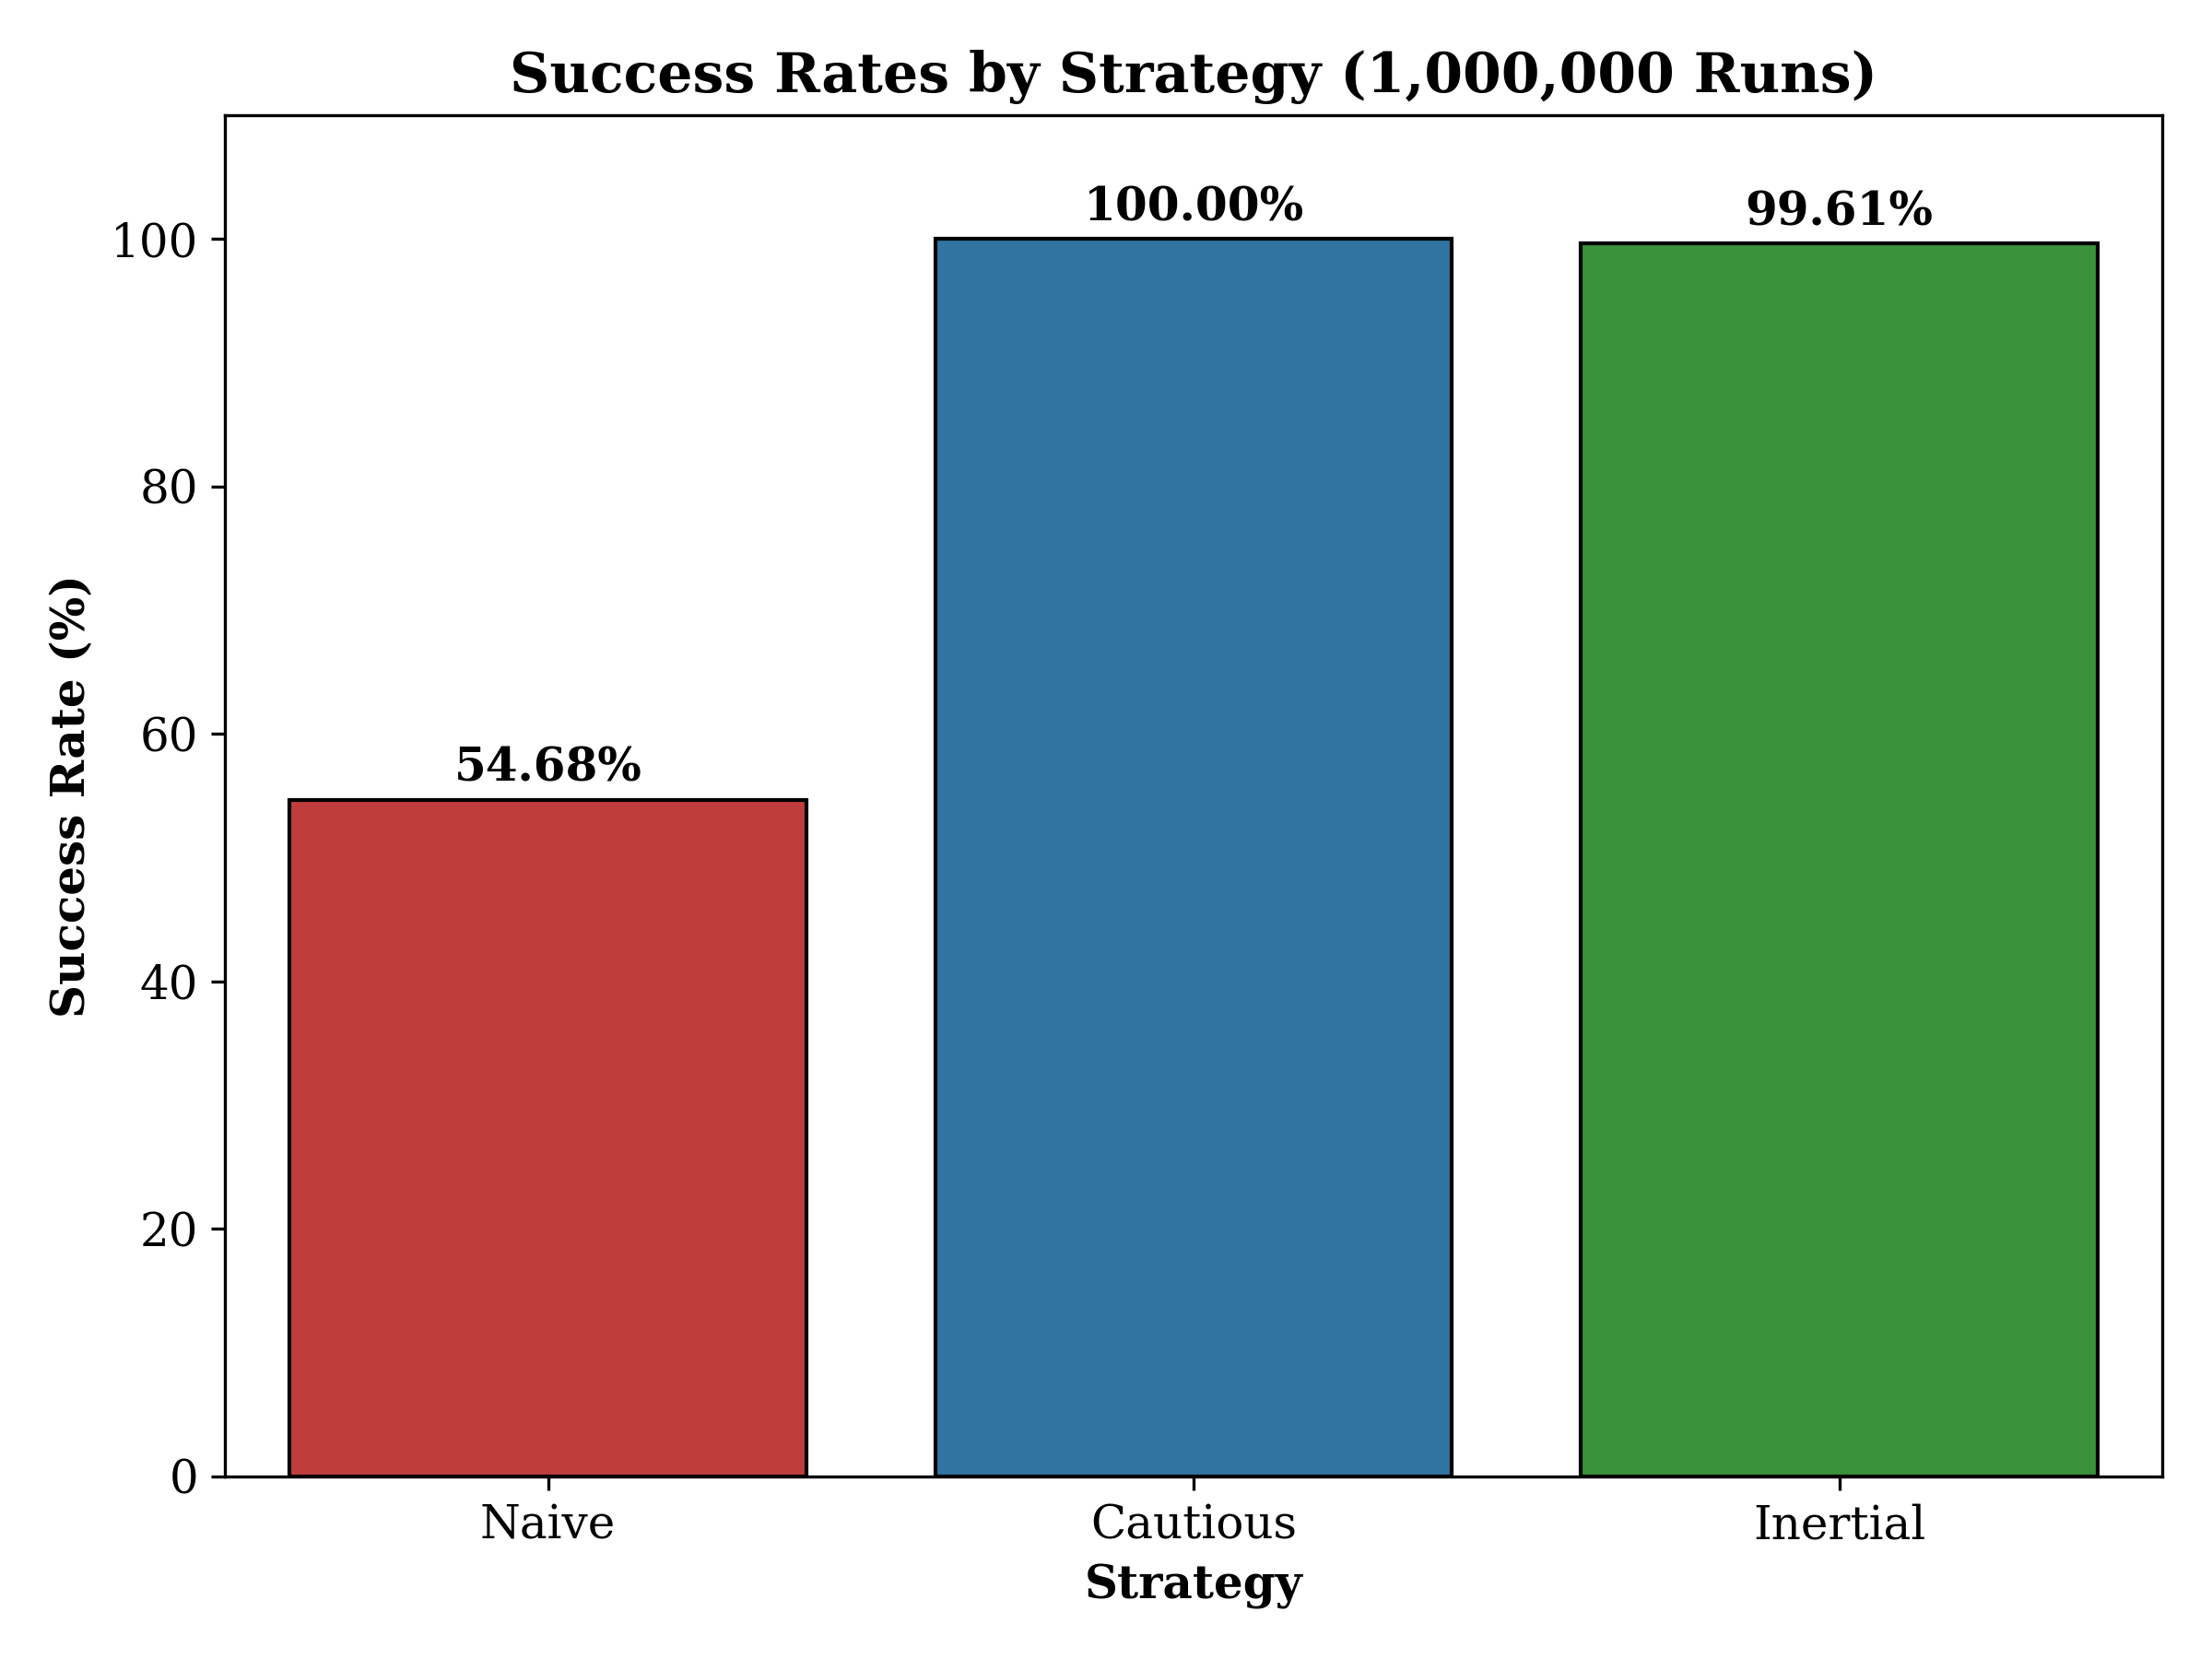
\includegraphics[width=\linewidth]{success_rates.png}
        \caption{שיעורי ההצלחה ב-$1,000,000$ מבוכים.}
        \label{fig:succ}
    \end{minipage}\hfill
    \begin{minipage}[t]{0.48\linewidth}
        \centering
        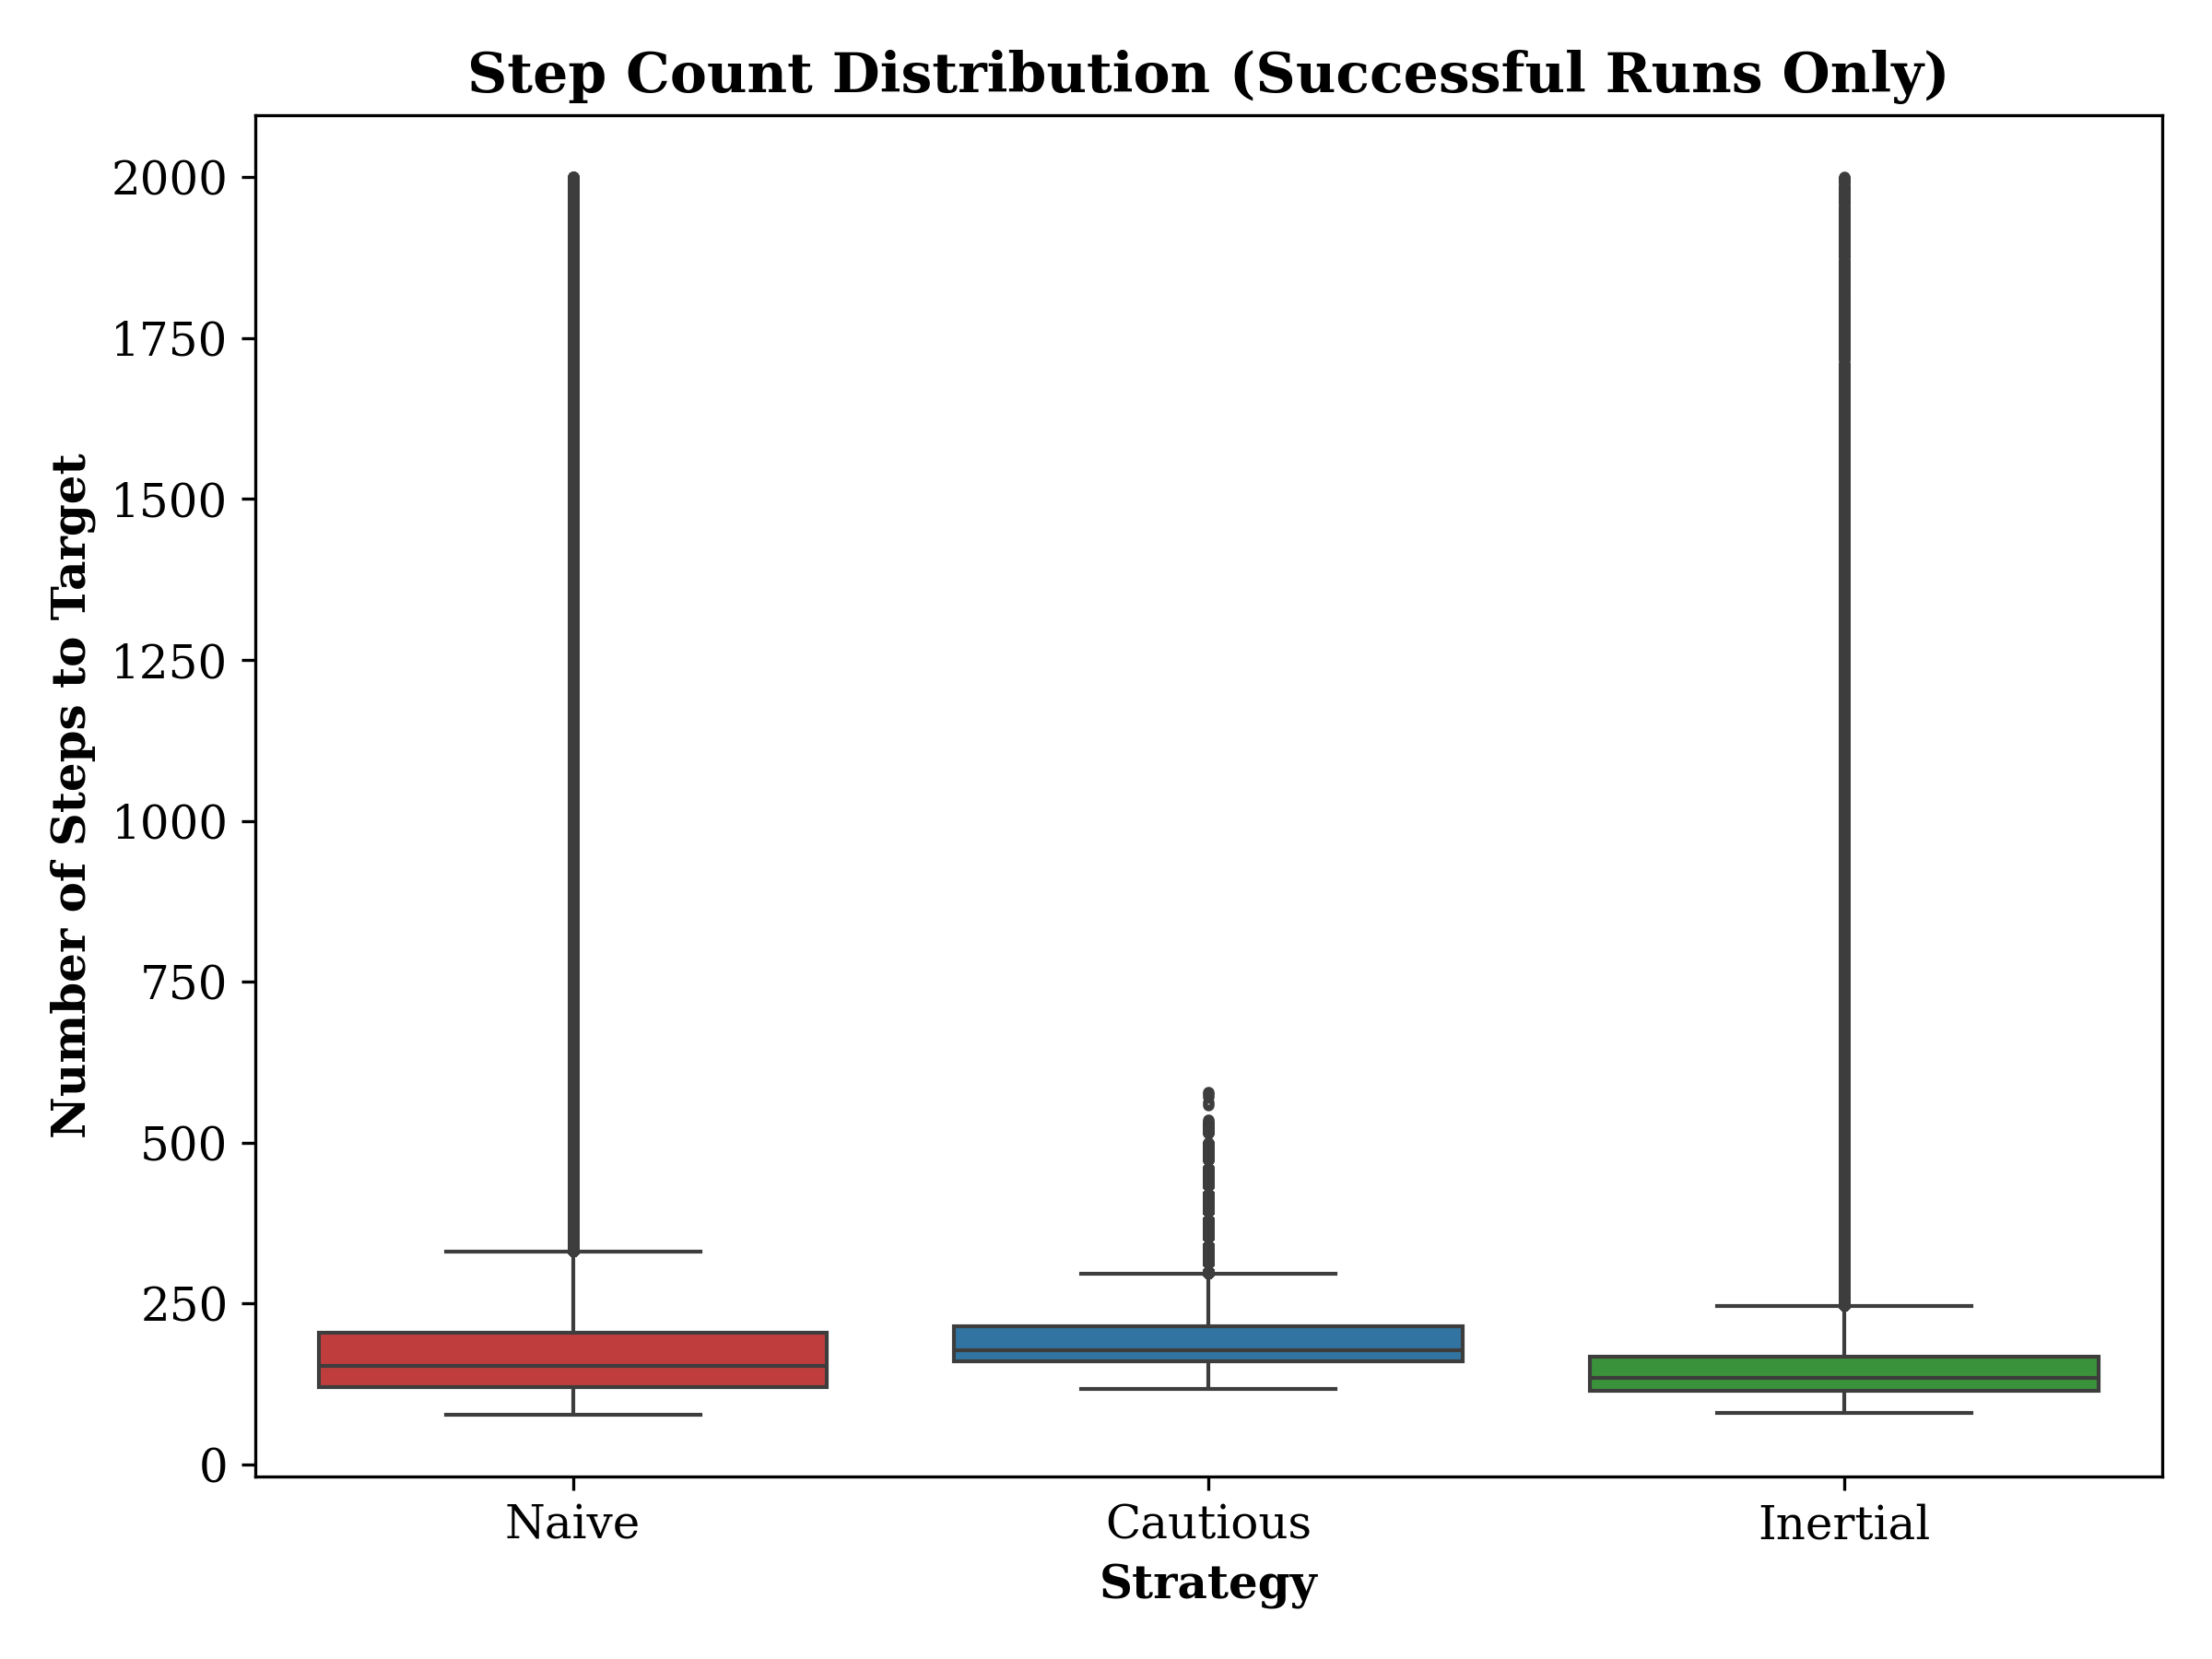
\includegraphics[width=\linewidth]{steps_distribution.png}
        \caption{התפלגות מספר הצעדים עד להגעה למטרה.}
        \label{fig:steps}
    \end{minipage}
\end{figure}

\noindent\textbf{שלוש המסקנות המרכזיות מהניסוי:}
\begin{enumerate}
    \item \textbf{קריסת הרובוט התמים (\foreignlanguage{english}{Naive}):} ללא מסנן האנומליות, הרובוט נכשל ב-$45.32\%$ מהמבוכים! באיור~\ref{fig:trap} ניתן לראות במסלול התכלת כיצד הרובוט פוגע במכשול האמצעי בצורת האות \foreignlanguage{english}{L} בזמן שהתוקף דולק, שומר סף מורעל גבוה ($i_H = 1.230$), ונלכד בהקפה אינסופית סביבו.
    \item \textbf{אמינות מושלמת של הרובוט הזהיר (\foreignlanguage{english}{Cautious}):} הרובוט הזהיר הצליח ב-$\mathbf{100.00\%}$ מההרצות (מיליון מתוך מיליון!), בדיוק כמו הרובוט שפעל ללא תוקף כלל, ובכך אישר בפועל את משפט~\ref{thm:cautious}. המחיר של הזהירות הזו הוא זמן המתנה: הוא זקוק בממוצע ל-$193.0$ צעדים לעומת $132.6$ צעדים ללא תקיפה (תוספת של $60.4$ צעדי המתנה בממוצע).
    \item \textbf{דילמת המהירות מול הבטיחות ברובוט האינרציאלי (\foreignlanguage{english}{Inertial}):} הרובוט האינרציאלי שממשיך ללכת בזמן תקיפה חוסך $20.5\%$ ממספר הצעדים לעומת הרובוט הזהיר ($153.4$ לעומת $193.0$ צעדים) ומצליח ב-$99.61\%$ מהמבוכים. אך ב-$0.39\%$ מהמקרים ($3,877$ מבוכים מתוך מיליון) הוא נכשל בגלל תופעת ה\textbf{תהודה} שהוכחנו בטענה~\ref{prop:resonance}! באיור~\ref{fig:trap} רואים זאת בבירור במסלול הירוק: הרובוט האינרציאלי נחלץ בהצלחה מהמכשול הראשון, אך במכשול המלבני העליון זמן ההקפה שלו מסתנכרן עם מחזור ה-$40$ צעדים של התוקף — בכל פעם שהוא מגיע לפינה הימנית-עליונה שממנה צריך לעזוב למטרה, התוקף נדלק ל-$10$ צעדים, והרובוט מפספס את היציאה שוב ושוב.
\end{enumerate}

\begin{figure}[H]
    \centering
    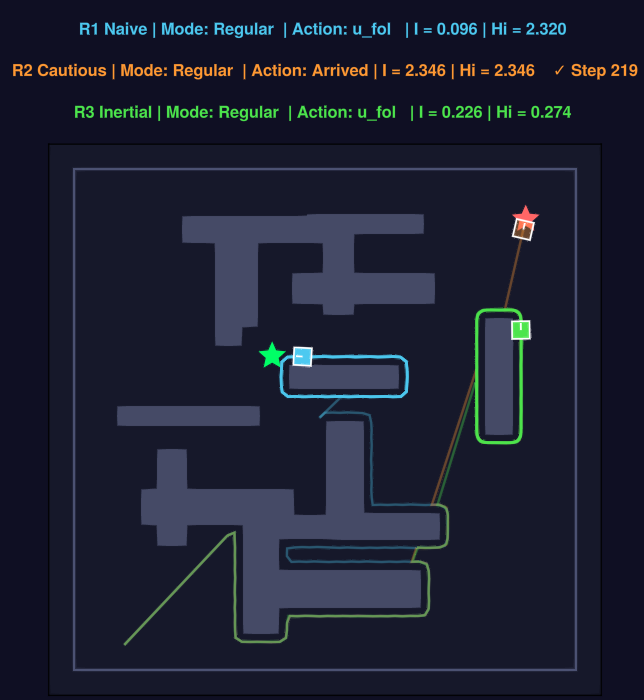
\includegraphics[width=0.72\linewidth]{simulation_trap.png}
    \caption{דוגמה אמיתית מתוך הסימולציה שבה רואים את שלושת הרובוטים באותו מבוך: \textbf{התמים (תכלת)} מורעל ונלכד במכשול ה-\foreignlanguage{english}{L} במרכז; \textbf{האינרציאלי (ירוק)} נלכד בלולאת תהודה מסונכרנת סביב המלבן העליון; ו\textbf{הזהיר (כתום)} עוצר בזמן ההפרעות ומגיע למגדל המטרה (הכוכב האדום) תוך $137$ צעדים. \textbf{[לצפייה בסרטון האנימציה של ההרצה צעד-אחר-צעד: \href{run:simulation_trap_anim.gif}{לחצו כאן לפתיחת \foreignlanguage{english}{simulation\_trap\_anim.gif}} או פתחו את \href{run:accessible_paper_online.html}{גרסת ה-\foreignlanguage{english}{HTML} המקוונת}]}}
    \label{fig:trap}
\end{figure}

\begin{otherlanguage}{english}
\begin{thebibliography}{8}
\footnotesize
\setlength{\itemsep}{0pt}
\bibitem{lumelsky1987path}
V.~J. Lumelsky and A.~A. Stepanov, ``Path-planning strategies for a point mobile automaton moving amidst unknown obstacles of arbitrary shape,'' \textit{Algorithmica}, vol.~2, no.~1, pp.~403--430, 1987.

\bibitem{kamon1998tangentbug}
I.~Kamon, E.~Rimon, and E.~Rivlin, ``TangentBug: A range-sensor-based navigation algorithm,'' \textit{Int. J. Robot. Res.}, vol.~17, no.~9, pp.~934--953, 1998.

\bibitem{taylor2009ibug}
K.~Taylor and S.~M. LaValle, ``I-Bug: An intensity-based bug algorithm,'' in \textit{Proc. IEEE Int. Conf. Robot. Autom. (ICRA)}, 2009, pp.~3981--3986.

\bibitem{taylor2014intensity}
K.~Taylor and S.~M. LaValle, ``Intensity-based navigation with global guarantees,'' \textit{Auton. Robots}, vol.~36, no.~4, pp.~349--364, 2014.

\bibitem{kerns2014unmanned}
A.~J. Kerns, D.~P. Shepard, J.~A. Bhatti, and T.~E. Humphreys, ``Unmanned aircraft capture and control via GPS spoofing,'' \textit{J. Field Robot.}, vol.~31, no.~4, pp.~617--636, 2014.

\bibitem{psiaki2016gnss}
M.~L. Psiaki and T.~E. Humphreys, ``GNSS spoofing and detection,'' \textit{Proc. IEEE}, vol.~104, no.~6, pp.~1258--1270, 2016.

\bibitem{giraldo2018survey}
J.~Giraldo \textit{et al.}, ``A survey of physics-based attack detection in cyber-physical systems,'' \textit{ACM Comput. Surv.}, vol.~51, no.~4, Art.~no.~76, pp.~1--36, 2018.

\bibitem{basseville1993detection}
M.~Basseville and I.~V. Nikiforov, \textit{Detection of Abrupt Changes: Theory and Application}. Englewood Cliffs, NJ, USA: Prentice Hall, 1993.
\end{thebibliography}
\end{otherlanguage}

\end{document}
